\documentclass[11pt]{article}
\usepackage{graphicx} % Para insertar imágenes
\usepackage[margin=0.5in]{geometry} 
\usepackage{amsmath, amssymb, array,amsfonts,xcolor}
\usepackage{float}    % Para un mejor control de las ubicaciones de la imagen
\usepackage{algorithm} % Paquete para algoritmos
\usepackage{algpseudocode} % Paquete para escribir pseudocódigo

\begin{document}

\begin{minipage}{0.4\textwidth}
    \raggedleft 
    \textbf{\Large Pr\'actica Filtros} \\ % Cambia por tu propio texto
    Procesamiento de Imágenes \\ % Cambia por tu propio texto
    Kenet Chapet\'on \\ 
\end{minipage}
\begin{minipage}{0.5\textwidth}
    \flushright % Alinea la imagen a la derecha
    
\includegraphics[width=0.7\linewidth]{logo_dc.jpg} % Cambia por el nombre de tu imagen
\end{minipage}
\vspace{2em} % Espacio vertical adicional

Ejercicio 1 \\ 

a) Tenemos, $ x = [0,1,0,0,0,0] $ y $h = [0,2,1,0,0]$ \\

Para realizar la convolución de forma visual debemos rotar a h: 

\[
\begin{array}{ccccccccccc}
x: & & & 0 & 1 & 0 & 0 & 0 & 0  \\
rotated(h):  & 0 & 0 & 1 & 2 & 0 & & \\
x * h:  & & & & 2 &  &  &  &   \\
\end{array}
\]

\[
\begin{array}{ccccccccccc}
x: & & & 0 & 1 & 0 & 0 & 0 & 0  \\
rotated(h):  & & 0 & 0 & 1 & 2 & 0   \\
x*h: & & & & 2 & 1 &  &  &   \\
\end{array}
\]

\[
\begin{array}{ccccccccccc}
x:  & & 0 & 1 & 0 & 0 & 0 & 0  \\
rotated(h):   &  & 0 & 0 & 1 & 2 & 0 \\
x*h:  & & & & 2 & 1 & 0 &  &   \\
\end{array}
\]

\[
\begin{array}{ccccccccccc}
x:  & & 0 & 1 & 0 & 0 & 0 & 0  \\
rotated(h):   &  &  & 0 & 0 & 1 & 2 &0 \\
x*h:  & & & & 2 & 1 & 0 & 0 &   \\
\end{array}
\]

\[
\begin{array}{ccccccccccc}
x:  & & 0 & 1 & 0 & 0 & 0 & 0  \\
rotated(h):   &  &  &  & 0 & 0 & 1 & 2 &0\\
x*h:  & & & & 2 & 1 & 0 & 0 & 0 &  \\
\end{array}
\]

\[
\begin{array}{ccccccccccc}
x:  & & 0 & 1 & 0 & 0 & 0 & 0  \\
rotated(h):  &  &  &  &  & 0 & 0 & 1 & 2 & 0 \\
x*h:  & & & & 2 & 1 & 0 & 0 & 0 & 0 &  \\
\end{array}
\]

b) 

\[
\begin{array}{ccccccccccc}
x: & & & 0 & 0 & 1 &0 &0 &0  \\
rotated(h): & 0 & 0 & 1 & 2 & 0 &  \\
x*h: & & & 0 & & & & &  \\
\end{array}
\]

\[
\begin{array}{ccccccccccc}
x: & & & 0 & 0 & 1 &0 &0 &0  \\
rotated(h): &  & 0 & 0 & 1 & 2 &0  \\
x*h: & & & 0 &2 & & & &  \\
\end{array}
\]

\[
\begin{array}{ccccccccccc}
x: & & & 0 & 0 & 1 &0 &0 &0  \\
rotated(h): &  &  & 0 & 0 &1 &2 &0  \\
x*h: & & & 0 &2 &1 & & &  \\
\end{array}
\]

\[
\begin{array}{ccccccccccc}
x: & & & 0 & 0 & 1 &0 &0 &0  \\
rotated(h): &  &  & & 0 &0 &1 &2 &0  \\
x*h: & & & 0 &2 &1 & 0& &  \\
\end{array}
\]

\[
\begin{array}{ccccccccccc}
x: & & & 0 & 0 & 1 &0 &0 &0  \\
rotated(h): &  &  & & 0 &0 &1 &2 &0  \\
x*h: & & & 0 &2 &1 & 0& &  \\
\end{array}
\]

\[
\begin{array}{ccccccccccc}
x: & & & 0 & 0 & 1 &0 &0 &0  \\
rotated(h): &  &  & &  &0 &0 &1 &2 &0  \\
x*h: & & & 0 &2 &1 & 0&0 &  \\
\end{array}
\]

\[
\begin{array}{ccccccccccc}
x: & & & 0 & 0 & 1 &0 &0 &0  \\
rotated(h): &  &  & &  & &0 &0 &1 &2 &0 \\
x*h: & & & 0 &2 &1 & 0&0 &0  \\
\end{array}
\]

c)

\[
\begin{array}{ccccccccccc}
x: & & & 0& 2& -1&0 &0 &0 \\
h: & 0& 1&2 &-1 &0 & \\
x*h: & & -2& & & & & \\
\end{array}
\]

\[
\begin{array}{ccccccccccc}
x: & & & 0& 2& -1&0 &0 &0 \\
rotated(h): & & 0&1 &2 &-1 &0 \\
x*h: & & -2&5 & & & & \\
\end{array}
\]

\[
\begin{array}{ccccccccccc}
x: & & & 0& 2& -1&0 &0 &0 \\
rotated(h): & & &0 &1 &2 &-1&0 \\
x*h: & & -2&5 & 0& & & \\
\end{array}
\]

\[
\begin{array}{ccccccccccc}
x: & & & 0& 2& -1&0 &0 &0 \\
rotated(h): & & & &0 &1 &2&-1 &0 \\
x*h: & & -2&5 & 0& -1& & \\
\end{array}
\]

\[
\begin{array}{ccccccccccc}
x: & & & 0& 2& -1&0 &0 &0 \\
rotated(h): & & & & &0 &1&2 &-1&0 \\
x*h: & & -2&5 & 0& -1& 0& \\
\end{array}
\]

\[
\begin{array}{ccccccccccc}
x: & & & 0& 2& -1&0 &0 &0 \\
rotated(h): & & & & & &0&1 &2&-1 &0 \\
x*h: & & -2&5 & 0& -1& 0& 0\\
\end{array}
\]

d) Aca tengo un problema de interpretación de como es $x$ e $h$, voy a suponer que tienen la siguiente forma, 

\[
x = \begin{bmatrix}
1 & 1 & 1  \\
1 & 1 & 1  \\
1 & 1 & 1  \\
\end{bmatrix}
\]

\[
h = \begin{bmatrix}
1 & 1 \\
1 & 1
\end{bmatrix}
\]

dando como resultado \\ 

\[
x*h = \begin{bmatrix}
    1 & 2 & 2 \\ 
    2 & 4 & 4 \\ 
    2 & 4 & 4
\end{bmatrix}
\]

Ejercicio 2

a,i) \\

Recordemos que estamos haciendo convolucion, por lo tanto debemos transponer el kernel para que sea visualmente amigable cada operacion y etapa 
\[
\begin{array}{cccccccc}
    \textcolor{violet}{0}&\textcolor{violet}{-1}&\textcolor{violet}{0}& & \\
    \textcolor{violet}{-1}&\textcolor{violet}{4}&\textcolor{violet}{-1}& & \\
    \textcolor{violet}{1}&\textcolor{violet}{-1}&\textcolor{violet}{0} \times 1 & 4 & 1 \\ 
    & & 2 & 5 & 3 & \\ 
\end{array}
\rightarrow
\begin{array}{ccccc}
    0 &  &  & &  \\
     &  &  & &  \\
     &  &  & &  \\
     &  &  & &  \\
\end{array}
\]

\[
\begin{array}{cccccccc}
    &\textcolor{violet}{0}&\textcolor{violet}{-1}& \textcolor{violet}{0}& \\
    &\textcolor{violet}{-1}&\textcolor{violet}{4}&\textcolor{violet}{-1} & \\
    &\textcolor{violet}{1}&\textcolor{violet}{-1}\times 1&\textcolor{violet}{0} \times 4 & 1 \\ 
    & & 2 & 5 & 3 & \\ 
\end{array}
\rightarrow
\begin{array}{ccccc}
    0 & -1 &  & &  \\
     &  &  & &  \\
     &  &  & &  \\
     &  &  & &  \\
\end{array}
\]

\[
\begin{array}{cccccccc}
    &&\textcolor{violet}{0}&\textcolor{violet}{-1}& \textcolor{violet}{0}& \\
    &&\textcolor{violet}{-1}&\textcolor{violet}{4}&\textcolor{violet}{-1} & \\
    &&\textcolor{violet}{1}\times 1&\textcolor{violet}{-1}\times 4&\textcolor{violet}{0} \times 1\\ 
    & & 2 & 5 & 3 & \\ 
\end{array}
\rightarrow
\begin{array}{ccccc}
    0 & -1 & -3 & &  \\
     &  &  & &  \\
     &  &  & &  \\
     &  &  & &  \\
\end{array}
\]
\[
\begin{array}{ccccccccc}
    &&&&\textcolor{violet}{0}&\textcolor{violet}{-1}& \textcolor{violet}{0}& \\
    &&&&\textcolor{violet}{-1}&\textcolor{violet}{4}&\textcolor{violet}{-1} & \\
    &&&1&\textcolor{violet}{1}\times 4&\textcolor{violet}{-1}\times 1&\textcolor{violet}{0} \\ 
    & & & 2 & 5 & 3 & \\ 
\end{array}
\rightarrow
\begin{array}{ccccc}
    0 & -1 & -3 &3 &  \\
     &  &  & &  \\
     &  &  & &  \\
     &  &  & &  \\
\end{array}
\]
\[
\begin{array}{cccccccccc}
    &&&&&\textcolor{violet}{0}&\textcolor{violet}{-1}& \textcolor{violet}{0}& \\
    &&&&&\textcolor{violet}{-1}&\textcolor{violet}{4}&\textcolor{violet}{-1} & \\
    &&&1&4&\textcolor{violet}{1}\times 1&\textcolor{violet}{-1}&\textcolor{violet}{0} \\ 
    & & & 2 & 5 & 3 & \\ 
\end{array}
\rightarrow
\begin{array}{ccccc}
    0 & -1 & -3 & 3&1\\
     &  &  & &  \\
     &  &  & &  \\
     &  &  & &  \\
\end{array}
\]
\[
\begin{array}{cccccccccc}
    \textcolor{violet}{0}&\textcolor{violet}{-1}& \textcolor{violet}{0}& &\\
    \textcolor{violet}{-1}&\textcolor{violet}{4}&\textcolor{violet}{-1}\times 1 &4&1& \\
    \textcolor{violet}{1}&\textcolor{violet}{-1}&\textcolor{violet}{0}\times 2 &5&3& \\ 
\end{array}
\rightarrow
\begin{array}{ccccc}
    0 & -1 & -3 & 3&1\\
    -1 &  &  & &  \\
     &  &  & &  \\
     &  &  & &  \\
\end{array}
\]
\[
\begin{array}{cccccccccc}
    &\textcolor{violet}{0}&\textcolor{violet}{-1}& \textcolor{violet}{0}& &\\
    &\textcolor{violet}{-1}&\textcolor{violet}{4}\times 1&\textcolor{violet}{-1}\times 4 &1& \\
    &\textcolor{violet}{1}&\textcolor{violet}{-1}\times 2&\textcolor{violet}{0}\times 5&3& \\ 
\end{array}
\rightarrow
\begin{array}{ccccc}
    0 & -1 & -3 & 3&1\\
    -1 & -2 &  & &  \\
     &  &  & &  \\
     &  &  & &  \\
\end{array}
\]
\[
\begin{array}{cccccccccc}
    &&\textcolor{violet}{0}&\textcolor{violet}{-1}& \textcolor{violet}{0}&\\
    &&\textcolor{violet}{-1}\times 1&\textcolor{violet}{4}\times 4&\textcolor{violet}{-1}\times 1&&\\
    &&\textcolor{violet}{1}\times 2&\textcolor{violet}{-1}\times 5&\textcolor{violet}{0}\times 3& \\ 
\end{array}
\rightarrow
\begin{array}{ccccc}
    0 & -1 & -3 & 3&1\\
    -1 & -2 & 11 & &  \\
     &  &  & &  \\
     &  &  & &  \\
\end{array}
\]
\[
\begin{array}{cccccccccc}
    &&&\textcolor{violet}{0}&\textcolor{violet}{-1}& \textcolor{violet}{0}&\\
    &&1&\textcolor{violet}{-1}\times 4&\textcolor{violet}{4}\times 1&\textcolor{violet}{-1}&&\\
    &&2&\textcolor{violet}{1}\times 5&\textcolor{violet}{-1}\times 3&\textcolor{violet}{0}& \\ 
\end{array}
\rightarrow
\begin{array}{ccccc}
    0 & -1 & -3 & 3&1\\
    -1 & -2 & 11 & 2&  \\
     &  &  & &  \\
     &  &  & &  \\
\end{array}
\]
\[
\begin{array}{cccccccccc}
    &&&&\textcolor{violet}{0}&\textcolor{violet}{-1}& \textcolor{violet}{0}&\\
    &&1&4&\textcolor{violet}{-1}\times 1&\textcolor{violet}{4}&\textcolor{violet}{-1}&&\\
    &&2&5&\textcolor{violet}{1}\times 3&\textcolor{violet}{-1}&\textcolor{violet}{0}& \\ 
\end{array}
\rightarrow
\begin{array}{ccccc}
    0 & -1 & -3 & 3&1\\
    -1 & -2 & 11 & 2&2\\
     &  &  & &  \\
     &  &  & &  \\
\end{array}
\]
\[
\begin{array}{cccccccccc}
    \textcolor{violet}{0}&\textcolor{violet}{-1}& \textcolor{violet}{0}\times 1&4&1&\\
    \textcolor{violet}{-1}&\textcolor{violet}{4}&\textcolor{violet}{-1}\times 2&5&3&\\
    \textcolor{violet}{1}&\textcolor{violet}{-1}&\textcolor{violet}{0}& \\ 
\end{array}
\rightarrow
\begin{array}{ccccc}
    0 & -1 & -3 & 3&1\\
    -1 & -2 & 11 & 2&2\\
    -2 &  &  & &  \\
     &  &  & &  \\
\end{array}
\]
\[
\begin{array}{cccccccccc}
    &\textcolor{violet}{0}&\textcolor{violet}{-1}\times 1& \textcolor{violet}{0}\times 4&1&\\
    &\textcolor{violet}{-1}&\textcolor{violet}{4}\times 2&\textcolor{violet}{-1}\times 5&3&\\
    &\textcolor{violet}{1}&\textcolor{violet}{-1}&\textcolor{violet}{0}& \\ 
\end{array}
\rightarrow
\begin{array}{ccccc}
    0 & -1 & -3 & 3&1\\
    -1 & -2 & 11 & 2&2\\
    -2 & 2 &  & &  \\
     &  &  & &  \\
\end{array}
\]
\[
\begin{array}{cccccccccc}
    &&\textcolor{violet}{0}\times 1&\textcolor{violet}{-1}\times 4& \textcolor{violet}{0}\times 1&\\
    &&\textcolor{violet}{-1}\times 2&\textcolor{violet}{4}\times 5&\textcolor{violet}{-1}\times 3&\\
    &&\textcolor{violet}{1}&\textcolor{violet}{-1}&\textcolor{violet}{0}& \\ 
\end{array}
\rightarrow
\begin{array}{ccccc}
    0 & -1 & -3 & 3&1\\
    -1 & -2 & 11 & 2&2\\
    -2 & 2 & 11 & &  \\
     &  &  & &  \\
\end{array}
\]
\[
\begin{array}{cccccccccc}
    &&1&\textcolor{violet}{0}\times 4&\textcolor{violet}{-1}\times 1& \textcolor{violet}{0}\\
    &&2&\textcolor{violet}{-1}\times 5&\textcolor{violet}{4}\times 3&\textcolor{violet}{-1}\\
    &&&\textcolor{violet}{1}&\textcolor{violet}{-1}&\textcolor{violet}{0}& \\ 
\end{array}
\rightarrow
\begin{array}{ccccc}
    0 & -1 & -3 & 3&1\\
    -1 & -2 & 11 & 2&2\\
    -2 & 2 & 11 & 6&  \\
     &  &  & &  \\
\end{array}
\]
\[
\begin{array}{cccccccccc}
    &&1&4&\textcolor{violet}{0}\times 1&\textcolor{violet}{-1}& \textcolor{violet}{0}\\
    &&2&5&\textcolor{violet}{-1}\times 3&\textcolor{violet}{4}&\textcolor{violet}{-1}\\
    &&&&\textcolor{violet}{1}&\textcolor{violet}{-1}&\textcolor{violet}{0}& \\ 
\end{array}
\rightarrow
\begin{array}{ccccc}
    0 & -1 & -3 & 3&1\\
    -1 & -2 & 11 & 2&2\\
    -2 & 2 & 11 & 6& -3 \\
     &  &  & &  \\
\end{array}
\]
\[
\begin{array}{cccccccccc}
    &&1&4&1&\\
    \textcolor{violet}{0}&\textcolor{violet}{-1}& \textcolor{violet}{0}\times 2 & 5&3\\
    \textcolor{violet}{-1}&\textcolor{violet}{4}&\textcolor{violet}{-1}\\
    \textcolor{violet}{1}&\textcolor{violet}{-1}&\textcolor{violet}{0}& \\ 
\end{array}
\rightarrow
\begin{array}{ccccc}
    0 & -1 & -3 & 3&1\\
    -1 & -2 & 11 & 2&2\\
    -2 & 2 & 11 & 6& -3 \\
    0 &  &  & &  \\
\end{array}
\]
\[
\begin{array}{cccccccccc}
    &&1&4&1&\\
    &\textcolor{violet}{0}&\textcolor{violet}{-1}\times 2& \textcolor{violet}{0}\times 5& 3\\
    &\textcolor{violet}{-1}&\textcolor{violet}{4}&\textcolor{violet}{-1}\\
    &\textcolor{violet}{1}&\textcolor{violet}{-1}&\textcolor{violet}{0}& \\ 
\end{array}
\rightarrow
\begin{array}{ccccc}
    0 & -1 & -3 & 3&1\\
    -1 & -2 & 11 & 2&2\\
    -2 & 2 & 11 & 6& -3 \\
    0 & -2 &  & &  \\
\end{array}
\]
\[
\begin{array}{cccccccccc}
    &&1&4&1&\\
    &&\textcolor{violet}{0}\times 2&\textcolor{violet}{-1}\times 5& \textcolor{violet}{0}\times 3\\
    &&\textcolor{violet}{-1}&\textcolor{violet}{4}&\textcolor{violet}{-1}\\
    &&\textcolor{violet}{1}&\textcolor{violet}{-1}&\textcolor{violet}{0}& \\ 
\end{array}
\rightarrow
\begin{array}{ccccc}
    0 & -1 & -3 & 3&1\\
    -1 & -2 & 11 & 2&2\\
    -2 & 2 & 11 & 6& -3 \\
    0 & -2 & -5 & &  \\
\end{array}
\]
\[
\begin{array}{cccccccccc}
    &&1&4&1&\\
    &&2&\textcolor{violet}{0}\times 3&\textcolor{violet}{-1}\times 5& \textcolor{violet}{0}&\\
    &&&\textcolor{violet}{-1}&\textcolor{violet}{4}&\textcolor{violet}{-1}\\
    &&&\textcolor{violet}{1}&\textcolor{violet}{-1}&\textcolor{violet}{0}& \\ 
\end{array}
\rightarrow
\begin{array}{ccccc}
    0 & -1 & -3 & 3&1\\
    -1 & -2 & 11 & 2&2\\
    -2 & 2 & 11 & 6& -3 \\
    0 & -2 & -5 & -3&  \\
\end{array}
\]
\[
\begin{array}{cccccccccc}
    &&1&4&1&\\
    &&2&3&\textcolor{violet}{0}\times 5&\textcolor{violet}{-1}&\textcolor{violet}{0}&\\
    &&&&\textcolor{violet}{-1}&\textcolor{violet}{4}&\textcolor{violet}{-1}\\
    &&&&\textcolor{violet}{1}&\textcolor{violet}{-1}&\textcolor{violet}{0}& \\ 
\end{array}
\rightarrow
\begin{array}{ccccc}
    0 & -1 & -3 & 3&1\\
    -1 & -2 & 11 & 2&2\\
    -2 & 2 & 11 & 6& -3 \\
    0 & -2 & -5 & -3& 0 \\
\end{array}
\]

ii) \\ 

\[
\begin{array}{cccccccc}
    \textcolor{violet}{3}&\textcolor{violet}{2}&\textcolor{violet}{1} \times 1 & 4 & 1 \\ 
    & & 2 & 5 & 3 & \\ 
\end{array}
\rightarrow
\begin{array}{ccccc}
    1 &  &  & &  \\
     &  &  & &  \\
\end{array}
\]
\[
\begin{array}{cccccccc}
    &\textcolor{violet}{3}&\textcolor{violet}{2}\times 1&\textcolor{violet}{1} \times 4 & 1  \\ 
    & & 2 & 5 & 3 & \\ 
\end{array}
\rightarrow
\begin{array}{ccccc}
    1 & 6 &  & &  \\
     &  &  & &  \\
\end{array}
\]
\[
\begin{array}{cccccccc}
    &&\textcolor{violet}{3}\times 1&\textcolor{violet}{2}\times 4&\textcolor{violet}{1} \times 1  \\ 
    & & 2 & 5 & 3 & \\ 
\end{array}
\rightarrow
\begin{array}{ccccc}
    1 & 6 & 12 & &  \\
     &  &  & &  \\
\end{array}
\]
\begin{center}
    ....
\end{center} 
\[
\begin{array}{cccccccc}
    1 & 4 &1 \\
    2&5&\textcolor{violet}{3}\times 3&\textcolor{violet}{2}&\textcolor{violet}{1}  \\ 
\end{array}
\rightarrow
\begin{array}{ccccc}
    1 & 6 & 12 & 14& 3 \\
    2 & 9 & 19 & 21& 9 \\
\end{array}
\]

iii) \\ 

\[
\begin{array}{cccccccc}
    \textcolor{violet}{-1} \\ 
    \textcolor{violet}{3} \\
    \textcolor{violet}{-2} \times 1 & 4 & 1 \\ 
     2 & 5 & 3 & \\ 
\end{array}
\rightarrow
\begin{array}{ccccc}
    -2 &  &  & &  \\
     &  &  & &  \\
\end{array}
\]
\[
\begin{array}{cccccccc}
    &\textcolor{violet}{-1} \\ 
    &\textcolor{violet}{3} \\
    1&\textcolor{violet}{-2} \times 4 &  1 \\ 
     2 & 5 & 3 & \\ 
\end{array}
\rightarrow
\begin{array}{ccccc}
    -2 & -8 &  & &  \\
     &  &  & &  \\
\end{array}
\] 
\begin{center}
    ....
\end{center}
\[
\begin{array}{cccccccc}
    1& 4 &  1 \\ 
    2 & 5 & 3 \times \textcolor{violet}{-1} \\
    && \textcolor{violet}{3}  \\
    && \textcolor{violet}{-2}  \\
\end{array}
\rightarrow
\begin{array}{ccc}
    -2 & -8 & -2 \\
    -1 & 2 & -3 \\
    5 & 11 & 8 \\
    -2 & -5 & -3 \\
\end{array}
\] 
b) \\ 

La justificación de esta fórmula se basa en cuántas posiciones puede ocupar el centro del kernel con respecto a la matriz original:

Cuando el kernel se desplaza sobre la matriz de entrada, cubre más espacio si sus dimensiones son grandes.
El resultado de la convolución contiene todos los desplazamientos, incluso aquellos donde el kernel solo toca parcialmente la matriz original.

En la primer etapa por ejemplo tenemos: \\

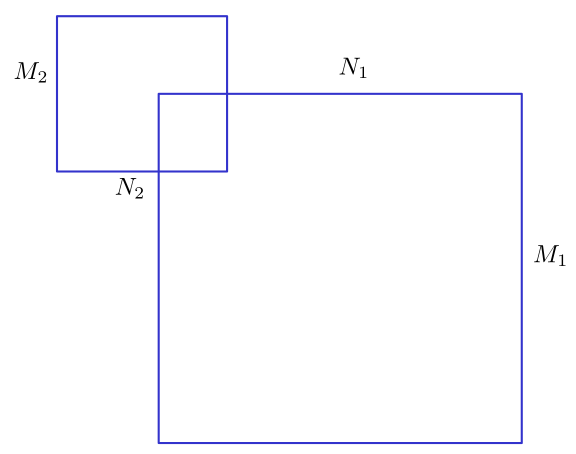
\includegraphics[width=0.3\linewidth]{etapa1.png} 

luego el kernel se movera $N_1$ hacia la derecha, entonces ...

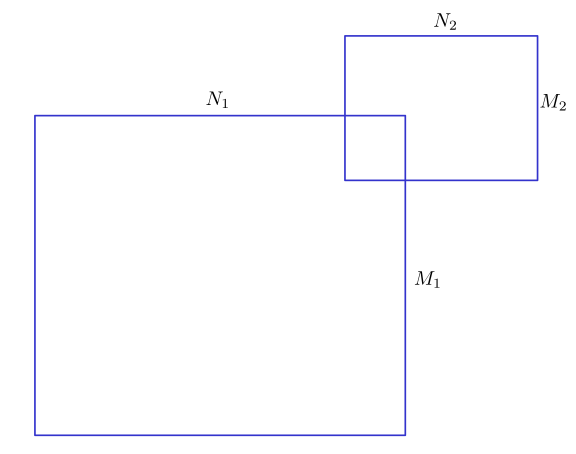
\includegraphics[width=0.3\linewidth]{etapa2.png} 

$N_2 - 1$, luego quedan $N_1 + N_2 - 1$ columnas, análogamente podemos hacerlo con las filas, donde quedan $M_1 + M_2 - 1$, finalmente la dimensión del array resultante sería $(M_1 + M_2 - 1,N_1 + N_2 - 1)$ \\

Ejercicio 3 

Entiendo que el ejercicio pide el algoritmo en pseudocodigo \\

% Definir el pseudocódigo
\begin{algorithm}
    \caption{Convolución2D(A,B)} % Título del algoritmo
    \begin{algorithmic}[1]
    \State \textbf{Input:} Matriz $A$ de dimensiones $M_1 \times N_1$, Matriz $B$ de dimensiones $M_2 \times N_2$
    \State \textbf{Output:} Matriz $C$ de dimensiones $(M_1 + M_2 - 1) \times (N_1 + N_2 - 1)$
    \State $M_r, N_r \leftarrow M_1 + M_2 - 1,  N_1 + N_2 - 1$
    \State  $C \leftarrow$ ceros$(M_r \times N_r)$
    
    \State  $A_{pad} \leftarrow ceros(M_1 + 2(M_2-1)) \times (N_1 + 2(N_2-1))$

    \State  \textbf{For} $i$ in $1...M_1$ \textbf{do}
    \State \hspace{1cm} \textbf{For} $j$ in $1...N_1$ \textbf{do}
    \State \hspace{2cm} $A_{pad}[i + (M_2-1), j + (N_2-1)] \leftarrow A[i,j]$ 
    \State \hspace{1cm} \textbf{End For}
    \State \textbf{end For}
    
    \State  \textbf{For} $i$ in $1...M_r$ \textbf{do}
    \State \hspace{1cm} \textbf{For} $j$ in $1...N_r$ \textbf{do}
    \State \hspace{2cm} region $\leftarrow A_{pad}[i:i+M_2,j:j+N_2]$
    \State \hspace{2cm} C $\leftarrow sum(region * B)$
    \State \hspace{1cm} \textbf{end For}
    \State \textbf{end For}
    
    \State \textbf{Return} $C$ 
    \end{algorithmic}
\end{algorithm}

Las pruebas estan en el codigo.\\ 

\newpage

Ejercicio 4. 

\end{document}
